%\documentclass[a4paper]{article}
\documentclass[a4paper,fleqn,12pt]{JMThesis}
%%% These are PDF packages needed to include PDF pictures
\usepackage[pdftex]{graphicx}
\DeclareGraphicsExtensions{.pdf}


\usepackage[OT2,T1]{fontenc}
\usepackage[english,serbian]{babel}

\newcommand{\cyr}{\fontencoding{OT2}\selectfont\selectlanguage{serbian}}
\newcommand{\latin}{\fontencoding{T1}\selectfont\selectlanguage{english}}

\usepackage{cmsrb}
% \usepackage[serbian]{babel}
\usepackage[utf8]{inputenc}

% \usepackage[OT2]{fontenc}
% \newcommand{\latin}{\fontencoding{T1}\selectfont}
\usepackage{substitutefont}

\renewcommand{\ch}{\v c}
\newcommand{\Ch}{\v C}
\renewcommand{\sh}{\v s}
\newcommand{\Sh}{\v S}
\newcommand{\zh}{\v z}
\newcommand{\Zh}{\v Z}


\renewcommand{\baselinestretch}{1}
\usepackage{amsfonts}
\usepackage{amssymb}
\usepackage{amsthm}
\usepackage{amsmath}
%\usepackage{gclc}
\usepackage{newlfont}
\usepackage{graphicx}
\usepackage{color}
\usepackage{verbatim,enumerate}
\usepackage{wasysym}
\usepackage{mdwlist}
\usepackage{multicol}
\usepackage{fancyhdr}
\usepackage{tocloft}
\usepackage[
backend=biber,
style=apa,
sorting=ynt
]{biblatex}

\usepackage[font=small,labelfont=bf]{caption}

\counterwithout{figure}{chapter}
\newcommand\DS{\displaystyle}
\newcommand\TS{\textstyle}
\newcommand{\konj}[1]{\overline {\rule {0pt}{7pt}{#1}}\,}
\oddsidemargin 1cm

\evensidemargin 0cm

\textwidth 15cm

\definecolor{Light}{gray}{.80}
\definecolor{Dark}{gray}{.20}

\pagestyle{headings}

\theoremstyle{plain}

\theoremstyle{definition}

 \newtheorem{pr}{Primer}
 \newtheorem{te}{Teorema}[chapter]
 \newtheorem{teo}{Teorema}[chapter]
 \newtheorem{lem}{Lema}[chapter]
 \newtheorem{lema}{Lema}[chapter]
 \newtheorem{po}{Posledica}
 \newtheorem{de}{Definicija}[chapter]
 \newtheorem{za}{Zadatak}
 \newtheorem{reza}{Reshenje}
 \newtheorem{fm}{F}

\newcommand{\dok}{\noindent \textit{Dokaz:}}

\newcommand{\zbn}{\sum_n}
\newcommand{\zbng}{\sum_{n=0}^\infty}
\newcommand{\zbk}{\sum_k}
\newcommand{\zbkg}{\sum_{k=0}^\infty}
\newcommand{\zbi}{\sum_i}
\newcommand{\zbig}{\sum_{i=0}^\infty}
\newcommand{\zbj}{\sum_j}
\newcommand{\zbjg}{\sum_{j=0}^\infty}
\newcommand{\zbtg}{\sum_{t=0}^\infty}
\newcommand{\osr}{\,_{\,\leftrightarrow}^{osr}\,}
\newcommand{\esr}{\,_{\,\leftrightarrow}^{esr}\,}
\newcommand{\piopt}{{\pi}_\text{\latin opt}}
\DeclareMathOperator{\EX}{\mathbb{E}}% expected value

\renewcommand*{\proofname}{Dokaz}
%\renewcommand*{\refname}{Literatura}
%\renewcommand{\figurename}{Slika.$ $ }
\theoremstyle{definition}

% Donji i gornji navosnici
\def\zn{,\kern-0.09em,}
\def\zng{'\kern-0.09em'}
\pagenumbering{roman}
\addbibresource{references.bib}

\begin{document}
% \thispagestyle{empty}
% \textcolor{white}{proba}
% \clearpage

\thispagestyle{empty}

\begin{center}
{\LARGE Ra\ch unarska gimnazija}
\end{center}
\vspace*{50mm}

\begin{center}
{\huge МАТУРСКИ РАД}

\vspace*{8pt}
{\Large Napredne tehnike programiranja}
\end{center}

\vspace*{10pt}
\begin{center}
{\LARGE Primena u\ch enja sa podsticajem za re\sh avanje Atari igara}
\end{center}

\vspace*{70mm}
\setlength{\columnsep}{50pt}
\begin{multicols}{2}
 {\noindent \Large Autor:
\\Ognjen Ne\sh ković}


{ \noindent \hfill \Large Mentor:\\
\hfill \phantom{aaaaaaaa}  dr Filip Marić}
\end{multicols}

\vfill
\begin{center}
{\Large Beograd, maj 2022.}
\end{center}

\newpage

\renewcommand{\contentsname}{Sadr\zh aj}
\thispagestyle{empty}
\pagenumbering{gobble}
\tableofcontents \clearpage

\pagenumbering{arabic}
\renewcommand{\chaptername}{}
\setcounter{page}{1}
\thispagestyle{plain}
{\Large Sa\zh etak}\\ 
Lorem ipsum dolor sit amet, consectetur adipiscing elit.

\chapter[Uvod]{Uvod}
\thispagestyle{plain}
\section[Osnove]{Osnove}
Još od davnina ljudi su se nadmetali u igranju igara poput šaha, 
kineske igre {\latin Go}, {\latin Backgammon} itd. 
U mnogim kulturama oni koji su bili najbolji u ovim igrama 
bili su izuzetno poštovani, pa bi neki ljudi posvećivali čak i 
čitav svoj život usavršavanju svoje strategije u nekoj od ovih 
igara. Stoga, dugo se smatralo da je sposobnost igranja ovih igara 
nešto jedinstveno za ljude i da je stvaranje mašine ili algoritma 
sposobnog da pobedi najboljeg šahistu ili drugog profesionalnog 
igrača gotovo nemoguće. \\
Ovaj izazov mučio je matematičare stotinama godina i ostao je 
neprevaziđen sve do 1997. godine kada je konačno računar 
{\latin (Deep blue)} prvi put pobedio najboljeg šahistu tog 
vremena Garija Kasparova {\latin (\cite{campbell2002deep})}. 
{\latin Deep blue} je koristio alfa-beta algoritam pretrage, 
heuristike, ekspertsko znanje i specijalni hardver napravljen 
kako bi probao što veći broj poteza po sekundi. 
Postojao je veći broj šahovskih mašina koje su prethodile 
{\latin Deep blue} mašini. Kako bi se razvio {\latin Deep blue} 
bilo je potrebno puno šahista, programera, vremena i novca. 
Dakle, jasno je da iako su velik uspeh, {\latin Deep blue} 
i njemu slične mašine nisu veoma generalne ili uopšte primenljive 
van vrlo specijalizovanog domena za koji su napravljene.\\
Velika prekretnica došla je sa razvojem neuronskih mreža, 
učenja sa podsticajem i hardvera. Sve ovo omogućilo je da se 
razviju generalni algoritmi koji bez velike modifikacije mogu 
naučiti da veoma dobro igraju veliki broj igara {\latin (\cite{mnih2015human})}. 
Sledeći veliki korak u mašinskom igranju igara došao je sa 
programom {\latin Alpha Go} koji je 2016. godine pobedio 
svetskog šampiona Li Sedola u igri Go. {\latin Alpha Go} je 
koristio učenje sa podsticajem, konvolucione neuronske mreže, 
Monte Karlo pretragu, takođe delimično je bio treniran na igrama 
koje su igrali profesionalni Go igrači {\latin (\cite{silver2017mastering})}. 
Godinu dana kasnije - 2017. godine objavljena je verzija {\latin Alpha Go-a} 
koja ne koristi ikakvo ekspertsko znanje - {\latin Alpha Go Zero}, 
koja postiže čak bolji rezultat od verzije trenirane sa ekspertskim 
igrama. Poslednji veliki napredak je program {\latin AlphaStar} 
koji igra stratešku video igru {\latin StarCraft II} gde pobeđuje 
najbolje igrače ove igre {\latin (\cite{vinyals2019grandmaster})}.\\
Glavna razlika između metoda korišćenih za rešavanje šaha 
(alfa-beta pretraga) i savremenih metoda je način kako se 
igra modeluje. U savremenim metodama učenja sa podsticajem 
problemi koje je potrebno rešiti predstavljaju se kao Markovljevi 
procesi odlučivanja. Ako se problem ovako prestavi u nekim 
jednostavnim slučajevima se može rešiti dinamičkim programiranjem, 
a za složenije slučajeve se rešenje može aproksimirati neuronskim 
mrežama.

\section[Motivacija]{Motivacija}
Igre ili opštije, problemi koji se mogu predstaviti kao Markovljevi procesi odlučivanja su od velikog teoretskog značaja za mašinsko učenje. Pored toga što donekle pružaju uvid u mogućnosti računara i razlike između ljudske i veštačke inteligencije, veliki broj procesa u stvarnosti poput problema optimalne kontrole (upravljanje robotima i mašinama), regulisanje sistema za hlađenje, kompresije videa itd. mogu se modelovati kao Markovljevi procesi odlučivanja. Složene igre pružaju dobar način da se granice savremenih metoda preciznije odrede, što primenu onda čini znatno lakšom. 
\section [Cilj Rada]{Cilj rada}
Cilj ovog rada je da se izlože metode učenja sa podsticajem od najjednostavnijih do složenijih. Uz ovo prikazani su problemi koji su rešivi svakom od metoda i problemi koji prevazilaze mogućnosti date metode, pa motivišu upotrebu neke složenije metode.

\chapter[Metode]{Metode}
\section[Uvod]{Uvod}
U narednom delu će biti razmatrane varijante Markovljevog procesa odlučivanja i rešenja koja su moguća za te varijante, pa je potrebno definisati Markovljev proces odlučivanja i uvesti potrebnu notaciju.
Markovljevi procesi odlučivanja su uopštenje Markovljevih lanaca sa dodatim akcijama, za definiciju markovljevog procesa potrebno je difinisati sledeće:
\begin{itemize}
	\item Skup stanja $S$
 	\item Skup akcija $A$ i $A_s$ - skup mogućih akcija u stanju $s$
	\item $P_a(s,s') = P(s_{t+1} = s' \mid s_t = s, a_t = a)$  - verovatnoću da se završi u stanju $s'$ ako je u stanju $s$ izvršena akcija $a$
	\item $R_a(s,s')$ - nagrada koja se ostvaruje kada se u stanju $s$ izvrši akcija $a$ i završi u stanju $s'$
 	\item Funkcija (politika) $\pi(s) : S \rightarrow A$ koja predstavlja igrača (onog koji donosi odluku), pa za dato stanje $s$ iz skupa stanja $S$ određuje akciju koju treba izvršiti 
\end{itemize}
Rešenje Markovljevog procesa odlučivanja je optimalna funkcija $\piopt$:
\[
	\text{\latin argmax}_{\piopt}\EX \left[ \zbtg \gamma^t R_{\piopt(s_t)}(s_t,s_{t+1}) \right]
\]
Posmatrajmo jednostavan Markovljev proces odlučivanja sa tri stanja ${S_0, S_1, S_2}$ i dve moguće akcije ${A_0, A_1}$ (slika 1).
\begin{figure}[!ht]
	\centering
	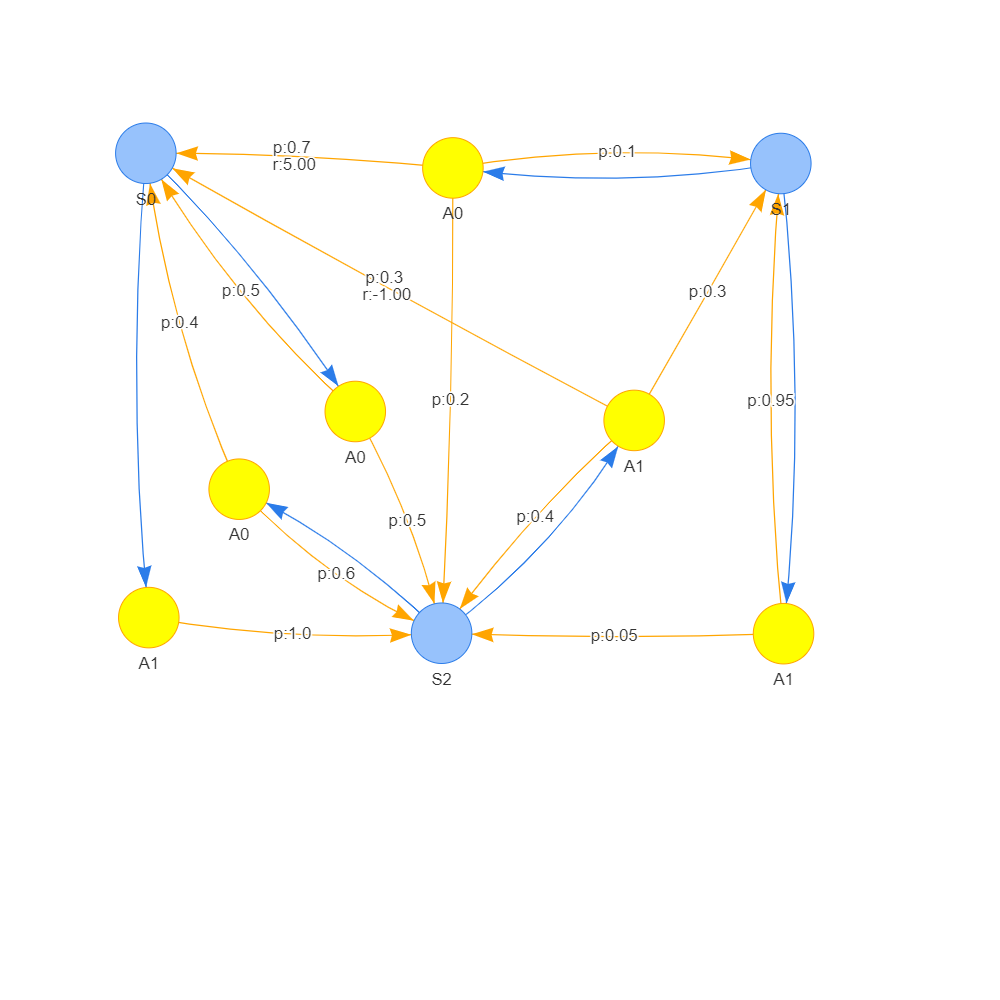
\includegraphics[scale=0.4]{../graph-visuals/example-mdp.png}
	\caption{Primer Markovljevog procesa odlučivanja}
\end{figure}

Primetimo da ukoliko se fiksira neka politika $\pi$, na primer $\pi(S_0)=A_0, \pi(S_1)=A_0, \pi(S_2)=A_1$ proces sa slike 1 postaje ekvivalentan novom procesu (slika 2).
\begin{figure}[!ht]
	\centering
	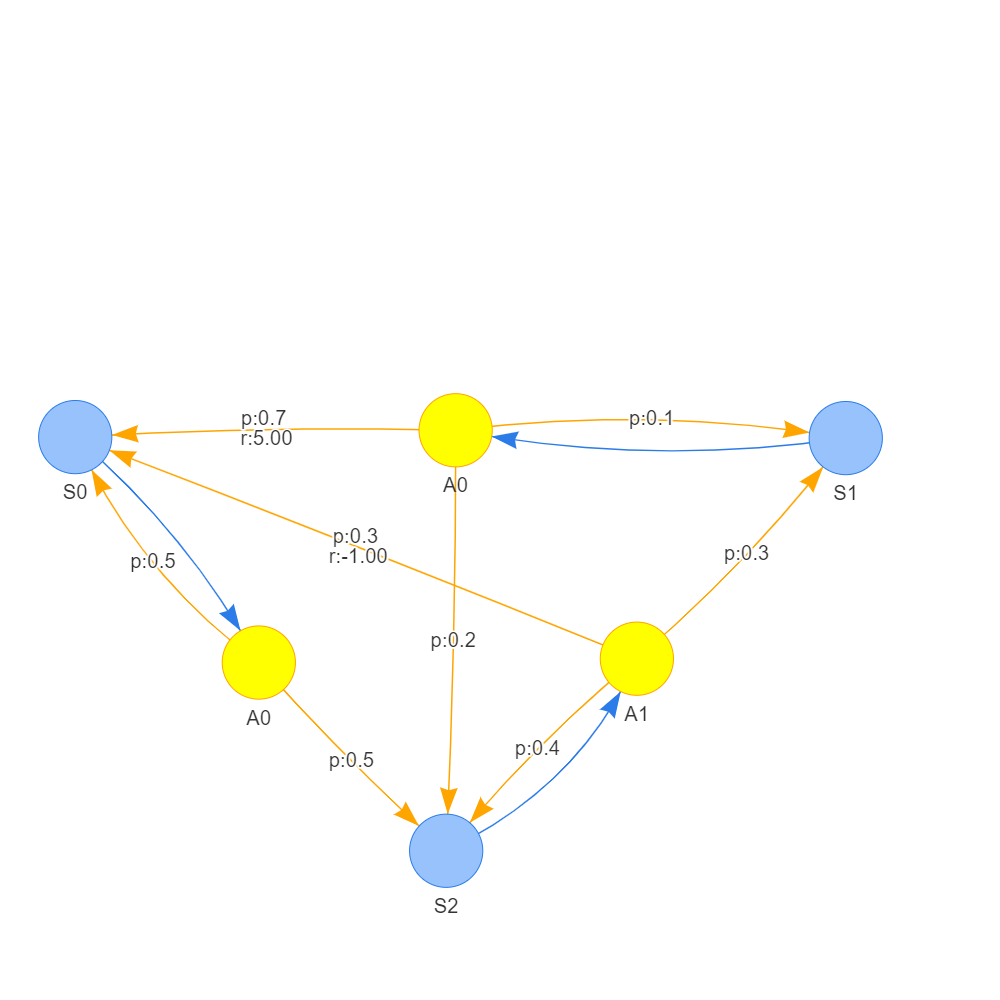
\includegraphics[scale=0.4]{../graph-visuals/example-mdp-given-policy.png}
	\caption{Markovljev proces pod politikom $\pi$}
\end{figure}

Dodatno, lako je videti da je tako dobijen proces (slika 2) ekvivalentan sledećem Markovljevom lancu, sa dodatim nagradama (slika 3).
\begin{figure}[!ht]
	\centering
	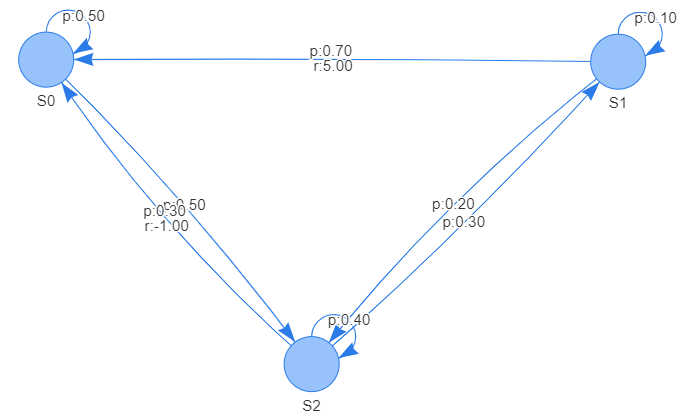
\includegraphics[scale=0.4]{../graph-visuals/example-mdp-given-policy-chain.png}
	\caption{Ekvivalentan Markovljev lanac sa nagradama}
\end{figure}
Kada je dat ovakav lanac, kao sa slike 3, postavlja se pitanje: kako efikasno odredti očekivanu nagradu u tonm lancu, ako je dato početno stanje ili verovatnoće da svako stanje bude početno. Ako je ovo moguće uraditi, onda je odmah dat efikasan način da se evaluira očekivana nagrada koja će biti ostvarena ako se koristi neka fiksna politika.\\

\subsection{Evaluacija politike ({\latin policy evaluation})}
Kada je politika fiksirana, traženje očekivane nagrade koja će biti ostvarena ako se prati data politika je ekvivalentna nalaženju očekivane nagrade u nekom markovljevom lancu. Prvo, uvedimo sledeću notaciju:
\begin{itemize}
	\item $S_t$ - Skup svih sekvenci dužine $t$. Na primer ako se iz stanja $N_0$ poseti stanje $N_1$, pa stanje $N_2$ itd. pa se na kraju poseti stanje $N_t$ sekvenca bi bila $(N_0, N_1, N_2, \cdots , N_t)$
 	\item $S_{t,u}$ - Skup svih sekvenci stanja dužine $t$ koje se završavaju sa stanjem $u$.
  	\item $T(u,v)$ - Verovatnoća da se iz stanja $u$ pređe u stanje $v$.
   	\item $p(s), s \in S_t$ - Verovatnoća da se neka sekvenca dogodi. Ako je data sekvenca $s=(N_0,N_1,N_2,\cdots , N_t)$ onda je $p(s) = T(N_0, N_1)\cdot T(N_1,N_2)\cdots T(N_{t-1},N_{t})$
    \item $R(u,v)$ - Nagrada kada se iz stanja $u$ završi u stanju $v$.
    \item $r(s), s \in S_t$ - Nagrada za datu sekvencu $s$. 
    \[ 
		\begin{split}
		r(s) &= R(N_0, N_1)+\gamma R(N_1,N_2) +\gamma^2 R(N_2,N_3) \cdots + \gamma^{t-1} R(N_{t-2},N_{t-1}) \\
		\gamma &< 1
		\end{split}
	\]
    \item $L(u,t)$ - Verovatnoća da se posle $t$ koraka završi u stanju $u$. 
	\[ 
		L(u,t) = \sum_{s \in S_{t,u}}p(s)
	\]
    \item $E_r(t)$ - Očekivana nagrada posle t koraka.
    \[
		E_r(t) = \sum_{s \in S_t}p(s)r(s)
	\]
\end{itemize}
\lem $L(u,t) = \sum_{v}T(v,u)L(v,t-1)$
\[
\begin{split}
	L(u,t) &= \sum_{s \in S_{t,u}}p(s)	\\
	L(u,t) &= \sum_{N_0, N_1, \cdots, N_{t-1}}T(N_0,N_1)\cdot T(N_1,N_2)\cdots T(N_{t-2},N_{t-1})\cdot T(N_{t-1},u)\\
	L(u,t) &= \sum_{v}\sum_{N_0, N_1,\cdots , N_{t-2}}T(N_0,N_1)\cdot T(N_1,N_2)\cdots T(N_{t-2},v) \cdot T(v,u)\\
	L(u,t) &= \sum_{v}T(v,u)\sum_{N_0, N_1,\cdots , N_{t-2}}T(N_0,N_1)\cdot T(N_1,N_2)\cdots T(N_{t-2},v)\\
	L(u,t) &= \sum_{v}T(v,u)L(v,t-1)
\end{split}
\]
Ako definišemo da je $L(t)$ vektorska funkcija, a $T$ matrica možemo prethodnu jednačinu zapisati elegantnije kao:
\[ L(t) = L(t-1)T \]
Kako je $L(0) = L_0$ gde je $L_0$ Verovatnoća da se počne iz svakog stanja. Lako se može pokazati da je:
\[ L(t) = L_0T^t \]
\lem $E_r(t) = E_r(t-1) + \gamma^{t-1}\sum_{u}\sum_{v}T(u,v)R(u,v)L(u,t)$
\[
\begin{split}
	E_r(t) &= \sum_{s \in S_t}p(s)r(s)	\\
	E_r(t) &= \sum_u \sum_{s' \in S_{t-1,u}}p(s')\sum_{v}T(u,v)(R(s') + \gamma^{t-1} R(u,v))\\
	E_r(t) &= \sum_u \sum_{s' \in S_{t-1,u}}p(s')(\sum_{v}T(u,v)R(s') + \gamma^{t-1} \sum_{v}T(u,v)R(u,v))\\
	E_r(t) &= \sum_u \sum_{s' \in S_{t-1,u}}p(s')(R(s')\sum_{v}T(u,v) + \gamma^{t-1} \sum_{v}T(u,v)R(u,v))\\
	E_r(t) &= \sum_u \sum_{s' \in S_{t-1,u}}p(s')(R(s')\cdot 1 + \gamma^{t-1} \sum_{v}T(u,v)R(u,v))\\
	E_r(t) &= \sum_u \sum_{s' \in S_{t-1,u}}p(s')(R(s') + \gamma^{t-1} \sum_{v}T(u,v)R(u,v))\\
	E_r(t) &= \sum_u \sum_{s' \in S_{t-1,u}}\left(p(s')R(s') + p(s')\gamma^{t-1}\sum_{v}T(u,v)R(u,v)\right)\\
	E_r(t) &= \sum_u \sum_{s' \in S_{t-1,u}}p(s')R(s') + \gamma^{t-1}\sum_u \sum_{s' \in S_{t-1,u}}p(s')\sum_{v}T(u,v)R(u,v)\\
	E_r(t) &= \sum_{s' \in S_{t-1}}p(s')R(s') + \gamma^{t-1}\sum_u \sum_{s' \in S_{t-1,u}}p(s')\sum_{v}T(u,v)R(u,v)\\
	E_r(t) &= E_r(t-1) + \gamma^{t-1}\sum_u \sum_{s' \in S_{t-1,u}}p(s')\sum_{v}T(u,v)R(u,v)\\
	E_r(t) &= E_r(t-1) + \gamma^{t-1}\sum_u \left(\sum_{v}T(u,v)R(u,v) \cdot \sum_{s' \in S_{t-1,u}}p(s')\right)\\
	E_r(t) &= E_r(t-1) + \gamma^{t-1}\sum_u \sum_{v}T(u,v)R(u,v) \cdot L(u,t)\\
\end{split}
\]
Dodatno možemo primetiti sledeće:
\[
	\sum_u \sum_{v}T(u,v)R(u,v) \cdot L(u,t) = \sum_u L(u,t)\sum_{v}T(u,v)R(u,v)
\]
Ukoliko definišemo $L(t)$ kao vektorsku funkciju, tako da je $L(t)_u$ verovatnoća da se u trenutku $t$ bude u stanju $u$ i primetimo da je $\sum_{v}T(u,v)R(u,v)$ konstantan vektor $\vec{c}$.
Možemo zapisati izraz kao:
\[
	E_r(t) = E_r(t-1) + \gamma^{t-1}\vec{L(t)} \cdot \vec{c}
\]  
Pa je lako videti da je:
\[
	\begin{split}
	E_r(t) &= \sum_{i=1}^{t}\gamma^{i-1}\vec{L(i)} \cdot \vec{c}\\
	E_r(t) &= \vec{c} \cdot \sum_{i=1}^{t}\gamma^{i-1}\vec{L(i)}
	\end{split}
\]
\medskip
Za aciklične markovljeve lance, odnosno za aperiodične matrice $T$ izračunavanje $E_r(t)$ za dovoljno veliko $t$ je dovoljno za nalaženje očekivane nagrade.
Međutim za periodične matrice $T$ je potrebno pokazati da $\lim_{t \to \infty}{E_r(t)}$ postoji.
\lem $\lim_{t \to \infty}{E_r(t)} = \text{const}$\\
Ako se u izraz $E_r(t) = \vec{c} \cdot \sum_{i=1}^{t}\gamma^{i-1}\vec{L(i-1)}$ zameni definicija za $\vec{L(i)}$ dobija se sledeći izraz:
\[
	\begin{split}
	E_r(t) &= \vec{c} \cdot \sum_{i=1}^{t}\gamma^{i-1}\vec{L_0}T^{i-1}\\
	E_r(t) &= \vec{c} \cdot \left( \vec{L_0} \cdot \sum_{i=1}^{t}\gamma^{i-1}T^{i-1}\right)\\
	\end{split}
\]
Uvedimo matricu $A = \gamma T$. Pa je prethodni izraz jednak: \\
\[
	\begin{split}
	E_r(t) &= \vec{c} \cdot \left( \vec{L_0} \cdot \sum_{i=1}^{t}A^i \right)\\
	\end{split}
\]
Pa je potrebno naći $\lim_{t \to \infty}{E_r(t)} = \vec{c} \cdot \left( \vec{L_0}\cdot \zbtg A^t \right)$.\\
$\zbtg A^t$ je Nojmanova serija primenjna na prostor $R^n$.\\
Dovoljan uslov za konvergenciju Nojmanove serije je da postoji norma tako da važi $||A|| < 1$.\\
Najlakše je odabrati $||A||_{\infty}$. Pa je lako videti da:
\[
	\begin{split}
	||A||_{\infty} &= \max_{i}\sum_{j}|A_{i,j}|\\
	||A||_{\infty} &= \gamma < 1\\
	\end{split}
\]
Pa znamo da suma konvergira, dodatno lako je pokazati da za sumu $S = \sum_{i=0}^{t}A^i$ važi $S(I - A) = I - A^{t-1}$.\\
Pa ukoliko postoji inverz $(I - A)^{-1}$ (što postoji kada Nojmanova serija konvergira) sledi da $S=(I - A^{t-1})(I-A)^{-1}$.\\
Kada $t \to \infty$ onda je $A^{t-1} = 0$. Pa je $S = I(I-A)^{-1} = (I-A)^{-1}$.\\
Čime je dokazano da $\lim_{t \to \infty}{E_r(t)} = \vec{c} \cdot \left( \vec{L_0} \cdot (I-A)^{-1} \right)$.

%%%%%%%%%%%%%%%%%%%%%%%%%%%%%%%%%%%%%%%%%%%%%%%%%%%%%%%%%%%%%%%%
%%%%%%%%%%%%%%%%%%%%%%%%%%%%%%%%%%%%%%%%%%%%%%%%%%%%%%%%%%%%%%%%
\chapter[Uvodni pojmovi]{Uvodni pojmovi}
\bigskip
\de Ovo je definicija. 

\de Ovo je \emph{druga} \textbf{definicija}.

\begin{figure}[ht]
	\includegraphics[scale=1]{resenje41.pdf}
	\figurename{Proba slike, sve je c1irilicom}
\end{figure}

%%%%%%%%%%%%%%%%%%%%%%%%%%%%%%%%%%%%%%%%%%%%%%%%%%%%%%%%%%%%%%%
%%%%%%%%%%%%%%%%%%%%%%%%%%%%%%%%%%%%%%%%%%%%%%%%%%%%%%%%%%%%%%%
%%%%%%%%%%%%%%%%%%%%%%%%%%%%%%%%%%%%%%%%%%%%%%%%%%%%%%%%%%%%%%%
%%%%%%%%%%%%%%%%%%%%%%%%%%%%%%%%%%%%%%%%%%%%%%%%%%%%%%%%%%%%%%%
\section[Topolo\sh ki prostori]{Topolo\sh ki prostori}
\medskip

\de 
\begin{enumerate}
\item[(1)]  Ovako se pi\sh e takozvana \emph{\latin inline} formula, $X\in\mathcal{O}$, koja se uklapa u tekst. 

\item[(2)] A ovako se pi\sh e formula koja je u zasebnom redu
\[
ax+by=c,\ \sum_{n=1}^{\infty} \frac{1}{n(n+1)} = \dots
\]

\item[(3)] Ukoliko \zh elite da jedna formula ima vi\sh e redova, jedan od na\ch ina da to postignete je 
\[
\begin{split}
 S &= puno formula, puno formula \\ &= 2.	
\end{split}
\]
\end{enumerate}

%%%%%%%%%%%%%%%%%%%%%%%%%%%%%%%%%%%%%%%%%%%%%%%%%%%%%%%%%%%%%%%
%%%%%%%%%%%%%%%%%%%%%%%%%%%%%%%%%%%%%%%%%%%%%%%%%%%%%%%%%%%%%%%
\section[Kratko ime]{Puno ime}
\medskip

\de \emph{Simpleks} 
\te  Za svako $n\geqslant 0$, sledec1a tvr\dj enja su
ekvivalentna i ta\ch na:
%%%%%%%%%%%%%%%%%%%%%%%%%%%%%%%%%%%%%%%%%%%%%%%%%%%%%%%%%%%%%%
\section[ Borsukov graf]{ Borsukov graf}

\bigskip

\teo  Za pozitivan realan broj $\alpha<2$, neka je
$B(n+1,\alpha)$ (beskona\ch an) 

\begin{proof}[Dokaz]
Pretpostavimo da va\zh i teorema Borsuk-Ulama i 
\end{proof}

 \clearpage \thispagestyle{empty} \textcolor{white}{proba}

%%%%%%%%%%%%%%%%%%%%%%%%%%%%%%%%%%%%%%%%%%%%%%%%%%%%%%%%%%%%%%


%\renewcommand*{\biblname}{}
\renewcommand\bibname{ Literatura}
 \addcontentsline{toc}{chapter}{ Literatura}
\latin
\printbibliography[title=Literatura]
\medskip


\end{document}
